%%
%% kit-prog-tutorial
%%
%% Slides for my Java programming tutorial at KIT using LaTeX beamer.
%%
%% Copyright (c) 2015-2016 YouniS Bensalah <younis.bensalah@gmail.com>
%%
%% This work is released to the public domain.
%% For the full copyright and license information, please view the LICENSE file.
%%

\documentclass[18pt]{beamer}

\usepackage{templates/beamerthemekit}

\usepackage[utf8]{inputenc}
\usepackage{hyperref}
\usepackage{listings}
\usepackage{xcolor}
\usepackage{colortbl}
\usepackage{array}
\usepackage{amsmath}
\usepackage{amssymb}
\usepackage{mathrsfs}
\usepackage{eurosym}

\titleimage{road}

\definecolor{lime}{HTML}{8FFF53}
\definecolor{darkgrey}{HTML}{5A5A5A}
\definecolor{awesome}{HTML}{FF2252}
\definecolor{lightgreen}{HTML}{E0FF98}

\newcommand{\tagline}{Search, Sort, Parse}

\newcommand{\quotes}[1]{``#1''}

\title[Programmieren\hspace{2.5pt}--\hspace{2.5pt}\tagline]{\tagline}
\subtitle{Programmieren~\textbar~Tutorium 32}

\author{YouniS Bensalah}
\date{30. Januar 2017}

\institute{Chair for Software Design and Quality}

\usepackage[citestyle=authoryear,bibstyle=numeric,hyperref,backend=biber]{biblatex}
\addbibresource{templates/example.bib}
\bibhang1em

\begin{document}

% remove annoying figure prefix in caption
\setbeamertemplate{caption}{\raggedright\insertcaption\par}

\selectlanguage{english}

\begin{frame}
    \titlepage
\end{frame}

% \begin{frame}{Heute}
%     \tableofcontents
% \end{frame}

\section{Suchen}

\begin{frame}{Suchen}
    \center
    \Huge{Suchen}
\end{frame}

\begin{frame}{Suchen}
    \begin{block}{}
        \textbf{Problem:}\\
        \textit{\quotes{Wie finde ich ein bestimmtes Element in einer Liste?}}
    \end{block}
    \vspace{.2in}
    \begin{center}
        \begin{tabular}{|c|c|c|c|c|c|c|c|}
            \hline
            4 & 2 & 3 & 9 & 7 & 13 & 6 & 10 \\
            \hline
        \end{tabular}
    \end{center}
\end{frame}

\subsection{Lineare Suche}

\begin{frame}{Lineare Suche}
    \begin{itemize}
        \item Erster (naiver) Ansatz: \textbf{Lineare Suche}
        \item Idee: Ein Element nach dem anderen anschauen und vergleichen
    \end{itemize}
\end{frame}

\begin{frame}[fragile]{Lineare Suche: Java-Code}
    \begin{exampleblock}{}
        \begin{lstlisting}[language=Java]
int linearSearch(int needle, int[] haystack) {
    for (int i = 0; i < haystack.length; i++) {
        if (haystack[i] == needle) {
            return i;
        }
    }
    return -1;
}
        \end{lstlisting}

    \end{exampleblock}

\end{frame}

\begin{frame}{Lineare Suche}
    \begin{itemize}
        \item Laufzeit: $\mathcal{O}(n)$
        \item Für beliebige Listen geht es nicht wirklich besser
    \end{itemize}
\end{frame}

\begin{frame}{Lineare Suche}
    \begin{itemize}
        \item Schade\dots
    \end{itemize}
\end{frame}


\subsection{Binäre Suche}

\begin{frame}{Binäre Suche}
    \begin{itemize}
        \item Ansatz: Suche auf einer vorsortierten Liste
        \item Idee: Teile die Liste in zwei Hälften und entscheide, in welcher der beiden Teillisten das gesuchte Element liegt und verwerfe die andere\\
        Dann wiederhole den Vorgang auf der übrigen Liste
        \item \textit{Divide and conquer}
    \end{itemize}
\end{frame}

\begin{frame}[fragile]{Binäre Suche: Java-Code}
    \begin{exampleblock}{}
        \begin{lstlisting}[language=Java,basicstyle=\scriptsize,basicstyle=\scriptsize]
int binarySearch(int needle, int[] haystack, int from, int to) {
    if (to > from) {
        int mid = (from + to) / 2;
        if (needle < haystack[mid]) {
            return binarySearch(needle, haystack, from, mid - 1);
        } else if (needle > haystack[mid]) {
            return binarySearch(needle, haystack, mid + 1, to);
        } else {
            return mid;
        }
    }
    return -1;
}
        \end{lstlisting}
    \end{exampleblock}
\end{frame}

\begin{frame}{Binäre Suche: Beispiel}
    Suche: \textbf{\alert{9}}
    \begin{center}
        \begin{tabular}{|c|c|c|c|c|c|c|c|c|c|c|c|c|c|c|c|}
            \hline
            \cellcolor{lightgreen}{3} & \cellcolor{lightgreen}{4} & \cellcolor{lightgreen}{4} & \cellcolor{lightgreen}{5} & \cellcolor{lightgreen}{6} & \cellcolor{lightgreen}{7} & \cellcolor{lightgreen}{9} & \cellcolor{lightgreen}{10} & \cellcolor{lightgreen}{11} & \cellcolor{lightgreen}{14} & \cellcolor{lightgreen}{17} & \cellcolor{lightgreen}{22} & \cellcolor{lightgreen}{24} & \cellcolor{lightgreen}{29} & \cellcolor{lightgreen}{32} & \cellcolor{lightgreen}{42} \\
            \hline
        \end{tabular}
        \pause
        \begin{tabular}{|c|c|c|c|c|c|c|c|c|c|c|c|c|c|c|c|}
            \hline
            \cellcolor{lightgreen}{3} & \cellcolor{lightgreen}{4} & \cellcolor{lightgreen}{4} & \cellcolor{lightgreen}{5} & \cellcolor{lightgreen}{6} & \cellcolor{lightgreen}{7} & \cellcolor{lightgreen}{9} & \cellcolor{lightgreen}{10} & \cellcolor{lime}{11} & \cellcolor{darkgrey}{14} & \cellcolor{darkgrey}{17} & \cellcolor{darkgrey}{22} & \cellcolor{darkgrey}{24} & \cellcolor{darkgrey}{29} & \cellcolor{darkgrey}{32} & \cellcolor{darkgrey}{42} \\
            \hline
        \end{tabular}
        \pause
        \begin{tabular}{|c|c|c|c|c|c|c|c|c|c|c|c|c|c|c|c|}
            \hline
            \cellcolor{darkgrey}{3} & \cellcolor{darkgrey}{4} & \cellcolor{darkgrey}{4} & \cellcolor{lime}{5} & \cellcolor{lightgreen}{6} & \cellcolor{lightgreen}{7} & \cellcolor{lightgreen}{9} & \cellcolor{lightgreen}{10} & \cellcolor{darkgrey}{11} & \cellcolor{darkgrey}{14} & \cellcolor{darkgrey}{17} & \cellcolor{darkgrey}{22} & \cellcolor{darkgrey}{24} & \cellcolor{darkgrey}{29} & \cellcolor{darkgrey}{32} & \cellcolor{darkgrey}{42} \\
            \hline
        \end{tabular}
        \pause
        \begin{tabular}{|c|c|c|c|c|c|c|c|c|c|c|c|c|c|c|c|}
            \hline
            \cellcolor{darkgrey}{3} & \cellcolor{darkgrey}{4} & \cellcolor{darkgrey}{4} & \cellcolor{darkgrey}{5} & \cellcolor{darkgrey}{6} & \cellcolor{lime}{7} & \cellcolor{lightgreen}{9} & \cellcolor{lightgreen}{10} & \cellcolor{darkgrey}{11} & \cellcolor{darkgrey}{14} & \cellcolor{darkgrey}{17} & \cellcolor{darkgrey}{22} & \cellcolor{darkgrey}{24} & \cellcolor{darkgrey}{29} & \cellcolor{darkgrey}{32} & \cellcolor{darkgrey}{42} \\
            \hline
        \end{tabular}
        \pause
        \begin{tabular}{|c|c|c|c|c|c|c|c|c|c|c|c|c|c|c|c|}
            \hline
            \cellcolor{darkgrey}{3} & \cellcolor{darkgrey}{4} & \cellcolor{darkgrey}{4} & \cellcolor{darkgrey}{5} & \cellcolor{darkgrey}{6} & \cellcolor{darkgrey}{7} & \cellcolor{lime}{9} & \cellcolor{lightgreen}{10} & \cellcolor{darkgrey}{11} & \cellcolor{darkgrey}{14} & \cellcolor{darkgrey}{17} & \cellcolor{darkgrey}{22} & \cellcolor{darkgrey}{24} & \cellcolor{darkgrey}{29} & \cellcolor{darkgrey}{32} & \cellcolor{darkgrey}{42} \\
            \hline
        \end{tabular}
        \pause
        \begin{tabular}{|c|c|c|c|c|c|c|c|c|c|c|c|c|c|c|c|}
            \hline
            \cellcolor{darkgrey}{3} & \cellcolor{darkgrey}{4} & \cellcolor{darkgrey}{4} & \cellcolor{darkgrey}{5} & \cellcolor{darkgrey}{6} & \cellcolor{darkgrey}{7} & \cellcolor{awesome}{9} & \cellcolor{darkgrey}{10} & \cellcolor{darkgrey}{11} & \cellcolor{darkgrey}{14} & \cellcolor{darkgrey}{17} & \cellcolor{darkgrey}{22} & \cellcolor{darkgrey}{24} & \cellcolor{darkgrey}{29} & \cellcolor{darkgrey}{32} & \cellcolor{darkgrey}{42} \\
            \hline
        \end{tabular}
    \end{center}
\end{frame}


\begin{frame}{Binäre Suche}
    \begin{itemize}
        \item Laufzeit: $\mathcal{O}(log(n))$
        \item Die Liste muss \textbf{sortiert} sein
    \end{itemize}
\end{frame}

\section{Sortieren}

\begin{frame}{Sortieren}
    \center
    \Huge{Sortieren}
\end{frame}

\begin{frame}{Sortieren}
    \begin{block}{}
        \textbf{Problem:}\\
        \textit{\quotes{Wie sortiere ich nun eine Liste?}}
    \end{block}
    \vspace{.2in}
    \begin{center}
        \begin{tabular}{|c|c|c|c|c|c|c|c|}
            \hline
            4 & 2 & 3 & 9 & 7 & 13 & 6 & 10 \\
            \hline
        \end{tabular}
    \end{center}
\end{frame}

\subsection{Bubble Sort}

\begin{frame}{Bubble Sort}
    \begin{itemize}
        \item Ansatz: Vertausche zwei unsortierte benachbarte Elemente, solange bis die Liste sortiert ist
    \end{itemize}
    \vspace{.2in}
    \begin{figure}
        
\includegraphics[scale=.5]{img/BubbleSort.jpg}
    \end{figure}
\end{frame}

\begin{frame}[fragile]{Bubble Sort: Java-Code}
    \begin{exampleblock}{}
        \begin{lstlisting}[language=Java,basicstyle=\scriptsize,basicstyle=\scriptsize]
void bubbleSort(int[] list) {
    int n = list.length;
    int swap;
    boolean swapped = true;
    while (swapped) {
        swapped = false;
        for (int i = 1; i < n; i++) {
            if (list[i] < list[i-1]) {
                swap = list[i];
                list[i] = list[i - 1];
                list[i - 1] = swap;
                swapped = true;
            }
        }
        n--;
    }
}
        \end{lstlisting}
    \end{exampleblock}
\end{frame}

\begin{frame}{Bubble Sort}
    \begin{itemize}
        \item Laufzeit: $\mathcal{O}(n^2)$
        \item Sehr naiver Algorithmus, allerdings gut, wenn die Liste quasi schon sortiert ist
        \item Ansonsten miserabel
    \end{itemize}
\end{frame}

\subsection{Selection Sort}

\begin{frame}{Selection Sort}
    \begin{itemize}
        \item Ansatz: Suche immer das kleinste Element der unsortierten Liste und füge es an den Rand der sortierten Liste ein
    \end{itemize}
    \vspace{.1in}
    \begin{figure}
        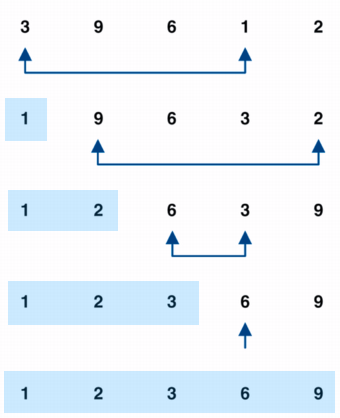
\includegraphics[scale=2.6]{img/SelectionSort.png}
    \end{figure}
\end{frame}

\begin{frame}[fragile]{Selection Sort: Java-Code}
    \begin{exampleblock}{}
        \begin{lstlisting}[language=Java,basicstyle=\scriptsize]
void selectionSort(int[] list) {
    int min, swap;
    for (int i = 1; i < list.length; i++) {
        min = i - 1;
        for (int j = i; j < list.length; j++) {
            if (list[j] < list[min]) {
                min = j;
            }
        }
        if (min != i - 1) {
            swap = list[i - 1];
            list[i - 1] = list[min];
            list[min] = swap;
        }
    }
}
        \end{lstlisting}
    \end{exampleblock}
\end{frame}

\begin{frame}{Selection Sort}
    \begin{itemize}
        \item Laufzeit: $\mathcal{O}(n^2)$
        \item Braucht \textit{immer} $\frac{n(n-1)}{2}$ Vergleiche!
    \end{itemize}
\end{frame}

\subsection{Insertion Sort}

\begin{frame}{Insertion Sort}
    \begin{itemize}
        \item Ansatz: Füge jedes Element der unsortierten Liste an die passende Stelle innerhalb der sortierten Liste
    \end{itemize}
    \vspace{.1in}
    \begin{figure}
        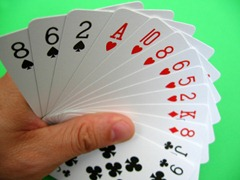
\includegraphics[scale=0.8]{img/InsertionSort.jpg}
    \end{figure}
\end{frame}

\begin{frame}[fragile]{Insertion Sort: Java-Code}
    \begin{exampleblock}{}
        \begin{lstlisting}[language=Java,basicstyle=\scriptsize]
void insertionSort(int[] list) {
    int j, current;
    for (int i = 1; i < list.length; i++) {
        current = list[i];
        j = i - 1;
        while (j >= 0 && list[j] > current) {
            list[j + 1] = list[j--];
        }
        list[j + 1] = current;
    }
}
        \end{lstlisting}
    \end{exampleblock}
\end{frame}

\begin{frame}{Insertion Sort}
    \begin{itemize}
        \item Laufzeit: $\mathcal{O}(n^2)$
        \item Das Vorgehen ist mit der Sortierung eines Spielkartenblatts vergleichbar
    \end{itemize}
\end{frame}

\section{Parsen}

\begin{frame}{Parsen}
    \center
    \Huge{Parsen}
\end{frame}

\begin{frame}{Parsen}
    \begin{block}{}
        \textbf{Problem:}\\
        \textit{\quotes{Wie kann eine Zeichenkette in semantisch sinnvolle Teile\\ zerlegt werden?}}
    \end{block}
    \vspace{.2in}
    \begin{figure}
        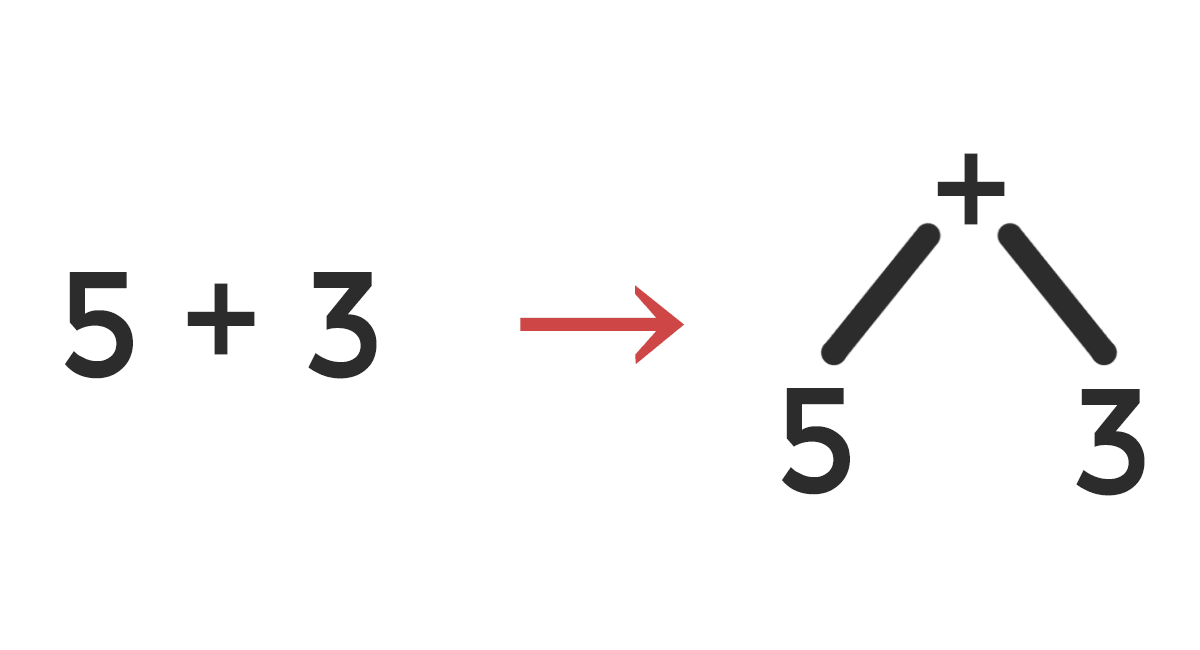
\includegraphics[scale=.1]{img/syntax-tree-basics.png}
    \end{figure}
\end{frame}

\subsection{Formale Grammatiken}

\begin{frame}{Crashkurs: Formale Grammatiken}
    \textit{Ganz formal\dots}
    \begin{block}{Definition}
        Eine Grammatik ist ein 4-Tupel $\mathcal{G} = (\mathcal{V}, \Sigma, \mathcal{P}, \mathcal{S})$ bestehend aus:
        \begin{itemize}
            \item $\mathcal{V}$, endliche Menge von \textbf{Variablen}
            \item $\Sigma$, endliche Menge von \textbf{Terminalsymbolen} (mit $\Sigma \cap \mathcal{V} = \emptyset$)
            \item $\mathcal{P} \subset (V \cup \Sigma)^+ \times (V \cup \Sigma)^*$, endliche Menge von \textbf{Produktionsregeln}
            \item $\mathcal{S} \in \mathcal{V}$, \textbf{Startsymbol}
        \end{itemize}
    \end{block}
\end{frame}

\begin{frame}{Crashkurs: Formale Grammatiken}
    \textit{Jetzt ein konkretes Beispiel für eine Grammatik\dots}
    \begin{block}{Klammerausdruck}
        \begin{itemize}
            \item $\mathcal{G} = (\mathcal{V} = \{\alert{X}, \alert{Y}\}, \quad \Sigma = \{\alert{(}, \alert{)}, \alert{\mathit{expr}}\}, \quad \mathcal{P}, \quad \mathcal{S} = \alert{X})$
            \item $\mathcal{P} = \{$\\
            $\quad X \longrightarrow (X)$\\
            $\quad X \longrightarrow XX$\\
            $\quad X \longrightarrow Y$\\
            $\quad Y \longrightarrow \mathit{expr}$\\
            $\}$
        \end{itemize}
    \end{block}
\end{frame}

\begin{frame}{Crashkurs: Formale Grammatiken}
    \begin{itemize}
        \item \textit{Dann sind folgende Wörter gültige Klammerausdrücke:}
        \begin{itemize}
            \item \texttt{expr}
            \item \texttt{(expr)}
            \item \texttt{(expr)(exprexpr)}
            \item \texttt{expr(expr(expr)(expr(expr)))expr((expr)expr)}
            \item \dots
        \end{itemize}
        \item \textit{Aber nicht sowas:}
        \begin{itemize}
            \item \texttt{)(}
            \item \texttt{expr()}
            \item \texttt{)(expr)}
            \item \texttt{term}
            \item \dots
        \end{itemize}
    \end{itemize}
\end{frame}

\subsection{Top-down Parsing}

\begin{frame}{Top-down Parsing}
    Idee:\\
    \begin{itemize}
        \item Verwende eine \textbf{formale Grammatik} um die gewünschte Sprache zu beschreiben
        \item Spalte die Eingabe in einzelne \textbf{Symbole} oder \textbf{Tokens}
        \item Ausgehend vom \textbf{Anfangssymbol} bestimme die nächste anzuwendende Produktion
    \end{itemize}
\end{frame}

\subsubsection{LL(1)-Parser}

\begin{frame}{LL(1)-Parser}
    \begin{itemize}
        \item Ein \textbf{LL(1)-Parser} ist ein einfacher \textbf{Top-down-Parser}
        \item Betrachte immer nur \textit{ein einziges Zeichen} (ganz links) um die nächste Regel zu entscheiden
        \item Grammatik darf dementsprechend \textbf{keine Konflikte bzgl. des ganz linken Symbols} haben (sonst siehe \quotes{Links-Faktorisierung}),
        da sonst mehrere Produktionen in Frage kommen und der Parser nicht mehr entscheiden kann, welche davon als nächstes angewandt werden soll
    \end{itemize}
\end{frame}

\begin{frame}{LL(1)-Parser: Beispiel}
    \textit{Ein konkretes Beispiel\dots}
    \begin{exampleblock}{LL(1)-Grammatik}
        \begin{itemize}
            \item $\mathcal{G} = (\mathcal{V} = \{\alert{X}, \alert{Y}\}, \quad \Sigma = \{\alert{(}, \alert{)}, \alert{+}, \alert{\mathit{a}}\}, \quad \mathcal{P}, \quad \mathcal{S} = \alert{X})$
            \item $\mathcal{P} = \{$\\
            $\quad X \longrightarrow Y$\\
            $\quad X \longrightarrow (X+Y)$\\
            $\quad Y \longrightarrow \mathit{a}$\\
            $\}$
        \end{itemize}
    \end{exampleblock}
    \vspace{.2in}
    \textbf{Eingabe:}\\
    \vspace{.1in}
    \texttt{((a+a)+a)}\\
\end{frame}

\begin{frame}{LL(1)-Parser: Beispiel}
    \begin{columns}[c]
        \column{.6\textwidth}
        \begin{itemize}
            \item Eingabe:\\
            \vspace{.1in}
            \texttt{((a+a)+a)}\\
            \vspace{.2in}
            \item Produktionen:\\
            \vspace{.1in}
                $\quad X \longrightarrow Y$\\
                $\quad X \longrightarrow (X+Y)$\\
                $\quad Y \longrightarrow \mathit{a}$\\
        \end{itemize}
        \column{.4\textwidth}
        \begin{itemize}
            \item Symbol-Stack:\\
            \vspace{.1in}
            X
        \end{itemize}
    \end{columns}
\end{frame}

\begin{frame}{LL(1)-Parser: Beispiel}
    \begin{columns}[c]
        \column{.6\textwidth}
        \begin{itemize}
            \item Eingabe:\\
            \vspace{.1in}
            \texttt{\alert{(}(a+a)+a)}\\
            \vspace{.2in}
            \item Produktionen:\\
            \vspace{.1in}
                $\quad X \longrightarrow Y$\\
                \alert{$\quad X \longrightarrow (X+Y)$}\\
                $\quad Y \longrightarrow \mathit{a}$\\
        \end{itemize}
        \column{.4\textwidth}
        \begin{itemize}
            \item Symbol-Stack:\\
            \vspace{.1in}
            \alert{X}
        \end{itemize}
    \end{columns}
\end{frame}

\begin{frame}{LL(1)-Parser: Beispiel}
    \begin{columns}[c]
        \column{.6\textwidth}
        \begin{itemize}
            \item Eingabe:\\
            \vspace{.1in}
            \texttt{((a+a)+a)}\\
            \vspace{.2in}
            \item Produktionen:\\
            \vspace{.1in}
                $\quad X \longrightarrow Y$\\
                $\quad X \longrightarrow (X+Y)$\\
                $\quad Y \longrightarrow \mathit{a}$\\
        \end{itemize}
        \column{.4\textwidth}
        \begin{itemize}
            \item Symbol-Stack:\\
            \vspace{.1in}
            $
            \begin{array}{c}
            $($ \\
            X \\
            + \\
            Y \\
            $)$
            \end{array}
            $
        \end{itemize}
    \end{columns}
\end{frame}

\begin{frame}{LL(1)-Parser: Beispiel}
    \begin{columns}[c]
        \column{.6\textwidth}
        \begin{itemize}
            \item Eingabe:\\
            \vspace{.1in}
            \texttt{\alert{(}(a+a)+a)}\\
            \vspace{.2in}
            \item Produktionen:\\
            \vspace{.1in}
                $\quad X \longrightarrow Y$\\
                $\quad X \longrightarrow (X+Y)$\\
                $\quad Y \longrightarrow \mathit{a}$\\
        \end{itemize}
        \column{.4\textwidth}
        \begin{itemize}
            \item Symbol-Stack:\\
            \vspace{.1in}
            $
            \begin{array}{c}
            $\alert{(}$ \\
            X \\
            + \\
            Y \\
            $)$
            \end{array}
            $
        \end{itemize}
    \end{columns}
\end{frame}

\begin{frame}{LL(1)-Parser: Beispiel}
    \begin{columns}[c]
        \column{.6\textwidth}
        \begin{itemize}
            \item Eingabe:\\
            \vspace{.1in}
            \texttt{(a+a)+a)}\\
            \vspace{.2in}
            \item Produktionen:\\
            \vspace{.1in}
                $\quad X \longrightarrow Y$\\
                $\quad X \longrightarrow (X+Y)$\\
                $\quad Y \longrightarrow \mathit{a}$\\
        \end{itemize}
        \column{.4\textwidth}
        \begin{itemize}
            \item Symbol-Stack:\\
            \vspace{.1in}
            $
            \begin{array}{c}
            X \\
            + \\
            Y \\
            $)$
            \end{array}
            $
        \end{itemize}
    \end{columns}
\end{frame}

\begin{frame}{LL(1)-Parser: Beispiel}
    \begin{columns}[c]
        \column{.6\textwidth}
        \begin{itemize}
            \item Eingabe:\\
            \vspace{.1in}
            \texttt{\alert{(}a+a)+a)}\\
            \vspace{.2in}
            \item Produktionen:\\
            \vspace{.1in}
                $\quad X \longrightarrow Y$\\
                \alert{$\quad X \longrightarrow (X+Y)$}\\
                $\quad Y \longrightarrow \mathit{a}$\\
        \end{itemize}
        \column{.4\textwidth}
        \begin{itemize}
            \item Symbol-Stack:\\
            \vspace{.1in}
            $
            \begin{array}{c}
            \alert{X} \\
            + \\
            Y \\
            $)$
            \end{array}
            $
        \end{itemize}
    \end{columns}
\end{frame}

\begin{frame}{LL(1)-Parser: Beispiel}
    \begin{columns}[c]
        \column{.6\textwidth}
        \begin{itemize}
            \item Eingabe:\\
            \vspace{.1in}
            \texttt{(a+a)+a)}\\
            \vspace{.2in}
            \item Produktionen:\\
            \vspace{.1in}
                $\quad X \longrightarrow Y$\\
                $\quad X \longrightarrow (X+Y)$\\
                $\quad Y \longrightarrow \mathit{a}$\\
        \end{itemize}
        \column{.4\textwidth}
        \begin{itemize}
            \item Symbol-Stack:\\
            \vspace{.1in}
            $
            \begin{array}{c}
            $($ \\
            X \\
            + \\
            Y \\
            $)$ \\
            + \\
            Y \\
            $)$
            \end{array}
            $
        \end{itemize}
    \end{columns}
\end{frame}

\begin{frame}{LL(1)-Parser: Beispiel}
    \begin{columns}[c]
        \column{.6\textwidth}
        \begin{itemize}
            \item Eingabe:\\
            \vspace{.1in}
            \texttt{\alert{(}a+a)+a)}\\
            \vspace{.2in}
            \item Produktionen:\\
            \vspace{.1in}
                $\quad X \longrightarrow Y$\\
                $\quad X \longrightarrow (X+Y)$\\
                $\quad Y \longrightarrow \mathit{a}$\\
        \end{itemize}
        \column{.4\textwidth}
        \begin{itemize}
            \item Symbol-Stack:\\
            \vspace{.1in}
            $
            \begin{array}{c}
            $\alert{(}$ \\
            X \\
            + \\
            Y \\
            $)$ \\
            + \\
            Y \\
            $)$
            \end{array}
            $
        \end{itemize}
    \end{columns}
\end{frame}

\begin{frame}{LL(1)-Parser: Beispiel}
    \begin{columns}[c]
        \column{.6\textwidth}
        \begin{itemize}
            \item Eingabe:\\
            \vspace{.1in}
            \texttt{a+a)+a)}\\
            \vspace{.2in}
            \item Produktionen:\\
            \vspace{.1in}
                $\quad X \longrightarrow Y$\\
                $\quad X \longrightarrow (X+Y)$\\
                $\quad Y \longrightarrow \mathit{a}$\\
        \end{itemize}
        \column{.4\textwidth}
        \begin{itemize}
            \item Symbol-Stack:\\
            \vspace{.1in}
            $
            \begin{array}{c}
            X \\
            + \\
            Y \\
            $)$ \\
            + \\
            Y \\
            $)$
            \end{array}
            $
        \end{itemize}
    \end{columns}
\end{frame}

\begin{frame}{LL(1)-Parser: Beispiel}
    \begin{columns}[c]
        \column{.6\textwidth}
        \begin{itemize}
            \item Eingabe:\\
            \vspace{.1in}
            \texttt{\alert{a}+a)+a)}\\
            \vspace{.2in}
            \item Produktionen:\\
            \vspace{.1in}
                \alert{$\quad X \longrightarrow Y$}\\
                $\quad X \longrightarrow (X+Y)$\\
                $\quad Y \longrightarrow \mathit{a}$\\
        \end{itemize}
        \column{.4\textwidth}
        \begin{itemize}
            \item Symbol-Stack:\\
            \vspace{.1in}
            $
            \begin{array}{c}
            \alert{X} \\
            + \\
            Y \\
            $)$ \\
            + \\
            Y \\
            $)$
            \end{array}
            $
        \end{itemize}
    \end{columns}
\end{frame}

\begin{frame}{LL(1)-Parser: Beispiel}
    \begin{columns}[c]
        \column{.6\textwidth}
        \begin{itemize}
            \item Eingabe:\\
            \vspace{.1in}
            \texttt{\alert{a}+a)+a)}\\
            \vspace{.2in}
            \item Produktionen:\\
            \vspace{.1in}
                $\quad X \longrightarrow Y$\\
                $\quad X \longrightarrow (X+Y)$\\
                \alert{$\quad Y \longrightarrow \mathit{a}$}\\
        \end{itemize}
        \column{.4\textwidth}
        \begin{itemize}
            \item Symbol-Stack:\\
            \vspace{.1in}
            $
            \begin{array}{c}
            \alert{Y} \\
            + \\
            Y \\
            $)$ \\
            + \\
            Y \\
            $)$
            \end{array}
            $
        \end{itemize}
    \end{columns}
\end{frame}

\begin{frame}{LL(1)-Parser: Beispiel}
    \begin{columns}[c]
        \column{.6\textwidth}
        \begin{itemize}
            \item Eingabe:\\
            \vspace{.1in}
            \texttt{\alert{a}+a)+a)}\\
            \vspace{.2in}
            \item Produktionen:\\
            \vspace{.1in}
                $\quad X \longrightarrow Y$\\
                $\quad X \longrightarrow (X+Y)$\\
                $\quad Y \longrightarrow \mathit{a}$\\
        \end{itemize}
        \column{.4\textwidth}
        \begin{itemize}
            \item Symbol-Stack:\\
            \vspace{.1in}
            $
            \begin{array}{c}
            \alert{a} \\
            + \\
            Y \\
            $)$ \\
            + \\
            Y \\
            $)$
            \end{array}
            $
        \end{itemize}
    \end{columns}
\end{frame}

\begin{frame}{LL(1)-Parser: Beispiel}
    \begin{columns}[c]
        \column{.6\textwidth}
        \begin{itemize}
            \item Eingabe:\\
            \vspace{.1in}
            \texttt{\alert{+}a)+a)}\\
            \vspace{.2in}
            \item Produktionen:\\
            \vspace{.1in}
                $\quad X \longrightarrow Y$\\
                $\quad X \longrightarrow (X+Y)$\\
                $\quad Y \longrightarrow \mathit{a}$\\
        \end{itemize}
        \column{.4\textwidth}
        \begin{itemize}
            \item Symbol-Stack:\\
            \vspace{.1in}
            $
            \begin{array}{c}
            \alert{+} \\
            Y \\
            $)$ \\
            + \\
            Y \\
            $)$
            \end{array}
            $
        \end{itemize}
    \end{columns}
\end{frame}

\begin{frame}{LL(1)-Parser: Beispiel}
    \begin{columns}[c]
        \column{.6\textwidth}
        \begin{itemize}
            \item Eingabe:\\
            \vspace{.1in}
            \texttt{\alert{a})+a)}\\
            \vspace{.2in}
            \item Produktionen:\\
            \vspace{.1in}
                $\quad X \longrightarrow Y$\\
                $\quad X \longrightarrow (X+Y)$\\
                \alert{$\quad Y \longrightarrow \mathit{a}$}\\
        \end{itemize}
        \column{.4\textwidth}
        \begin{itemize}
            \item Symbol-Stack:\\
            \vspace{.1in}
            $
            \begin{array}{c}
            \alert{Y} \\
            $)$ \\
            + \\
            Y \\
            $)$
            \end{array}
            $
        \end{itemize}
    \end{columns}
\end{frame}

\begin{frame}{LL(1)-Parser: Beispiel}
    \begin{columns}[c]
        \column{.6\textwidth}
        \begin{itemize}
            \item Eingabe:\\
            \vspace{.1in}
            \texttt{\alert{a})+a)}\\
            \vspace{.2in}
            \item Produktionen:\\
            \vspace{.1in}
                $\quad X \longrightarrow Y$\\
                $\quad X \longrightarrow (X+Y)$\\
                $\quad Y \longrightarrow \mathit{a}$\\
        \end{itemize}
        \column{.4\textwidth}
        \begin{itemize}
            \item Symbol-Stack:\\
            \vspace{.1in}
            $
            \begin{array}{c}
            \alert{a} \\
            $)$ \\
            + \\
            Y \\
            $)$
            \end{array}
            $
        \end{itemize}
    \end{columns}
\end{frame}

\begin{frame}{LL(1)-Parser: Beispiel}
    \begin{columns}[c]
        \column{.6\textwidth}
        \begin{itemize}
            \item Eingabe:\\
            \vspace{.1in}
            \texttt{\alert{)}+a)}\\
            \vspace{.2in}
            \item Produktionen:\\
            \vspace{.1in}
                $\quad X \longrightarrow Y$\\
                $\quad X \longrightarrow (X+Y)$\\
                $\quad Y \longrightarrow \mathit{a}$\\
        \end{itemize}
        \column{.4\textwidth}
        \begin{itemize}
            \item Symbol-Stack:\\
            \vspace{.1in}
            $
            \begin{array}{c}
            $\alert{)}$ \\
            + \\
            Y \\
            $)$
            \end{array}
            $
        \end{itemize}
    \end{columns}
\end{frame}

\begin{frame}{LL(1)-Parser: Beispiel}
    \begin{columns}[c]
        \column{.6\textwidth}
        \begin{itemize}
            \item Eingabe:\\
            \vspace{.1in}
            \texttt{\alert{+}a)}\\
            \vspace{.2in}
            \item Produktionen:\\
            \vspace{.1in}
                $\quad X \longrightarrow Y$\\
                $\quad X \longrightarrow (X+Y)$\\
                $\quad Y \longrightarrow \mathit{a}$\\
        \end{itemize}
        \column{.4\textwidth}
        \begin{itemize}
            \item Symbol-Stack:\\
            \vspace{.1in}
            $
            \begin{array}{c}
            \alert{+} \\
            Y \\
            $)$
            \end{array}
            $
        \end{itemize}
    \end{columns}
\end{frame}

\begin{frame}{LL(1)-Parser: Beispiel}
    \begin{columns}[c]
        \column{.6\textwidth}
        \begin{itemize}
            \item Eingabe:\\
            \vspace{.1in}
            \texttt{\alert{a})}\\
            \vspace{.2in}
            \item Produktionen:\\
            \vspace{.1in}
                $\quad X \longrightarrow Y$\\
                $\quad X \longrightarrow (X+Y)$\\
                \alert{$\quad Y \longrightarrow \mathit{a}$}\\
        \end{itemize}
        \column{.4\textwidth}
        \begin{itemize}
            \item Symbol-Stack:\\
            \vspace{.1in}
            $
            \begin{array}{c}
            \alert{Y} \\
            $)$
            \end{array}
            $
        \end{itemize}
    \end{columns}
\end{frame}

\begin{frame}{LL(1)-Parser: Beispiel}
    \begin{columns}[c]
        \column{.6\textwidth}
        \begin{itemize}
            \item Eingabe:\\
            \vspace{.1in}
            \texttt{\alert{a})}\\
            \vspace{.2in}
            \item Produktionen:\\
            \vspace{.1in}
                $\quad X \longrightarrow Y$\\
                $\quad X \longrightarrow (X+Y)$\\
                $\quad Y \longrightarrow \mathit{a}$\\
        \end{itemize}
        \column{.4\textwidth}
        \begin{itemize}
            \item Symbol-Stack:\\
            \vspace{.1in}
            $
            \begin{array}{c}
            \alert{a} \\
            $)$
            \end{array}
            $
        \end{itemize}
    \end{columns}
\end{frame}

\begin{frame}{LL(1)-Parser: Beispiel}
    \begin{columns}[c]
        \column{.6\textwidth}
        \begin{itemize}
            \item Eingabe:\\
            \vspace{.1in}
            \texttt{\alert{)}}\\
            \vspace{.2in}
            \item Produktionen:\\
            \vspace{.1in}
                $\quad X \longrightarrow Y$\\
                $\quad X \longrightarrow (X+Y)$\\
                $\quad Y \longrightarrow \mathit{a}$\\
        \end{itemize}
        \column{.4\textwidth}
        \begin{itemize}
            \item Symbol-Stack:\\
            \vspace{.1in}
            $
            \begin{array}{c}
            $\alert{)}$
            \end{array}
            $
        \end{itemize}
    \end{columns}
\end{frame}

\begin{frame}{LL(1)-Parser: Beispiel}
    \begin{columns}[c]
        \column{.6\textwidth}
        \begin{itemize}
            \item Eingabe:\\
            \vspace{.1in}
            $\emptyset$
            \vspace{.2in}
            \item Produktionen:\\
            \vspace{.1in}
                $\quad X \longrightarrow Y$\\
                $\quad X \longrightarrow (X+Y)$\\
                $\quad Y \longrightarrow \mathit{a}$\\
        \end{itemize}
        \column{.4\textwidth}
        \begin{itemize}
            \item Symbol-Stack:\\
            \vspace{.1in}
            $\emptyset$
        \end{itemize}
    \end{columns}
\end{frame}





\subsection{Regular Expressions}

\begin{frame}{Everybody stand back\dots}
    \begin{figure}
        
\includegraphics[scale=1.4]{img/regex_shirt.jpg}
    \end{figure}
\end{frame}



\begin{frame}{I'm about to know Regular Expressions}
    \begin{block}{Regular Expressions}
        \textbf{Reguläre Ausdrücke} sind Zeichenketten, die ein Muster zum \textit{Suchen} und \textit{Ersetzen} von Text beschreiben
    \end{block}

    \begin{itemize}
        \item Beispiele
        \begin{itemize}
            \item \textbf{Suche}: \textit{Alle Wörter, die auf \quotes{m} enden}
            \item \textbf{Ersetze}: \textit{Alle Wörter \quotes{keyboard} durch \quotes{leopard}}
            \item \textbf{Teste}: \textit{Enthält dieser Text ein Zeichen aus der Menge \quotes{0} \dots \quotes{9}?}
        \end{itemize}

    \end{itemize}

\end{frame}

\begin{frame}{Crashkurs: Java Regex}
    \begin{itemize}
        \item In Java: \texttt{java.util.regex.Matcher} und \texttt{java.util.regex.Pattern} oder \texttt{String.matches()}
        \item Regex sind sehr mächtig und können oft praktisch sein
        \begin{itemize}
            \item Einfaches Parsen
            \item Eingabe auf Gültigkeit checken
            \item Text nach Wort/Muster durchsuchen
        \end{itemize}
    \end{itemize}

\end{frame}



\begin{frame}[fragile]{Crashkurs: Java Regex}
    \begin{itemize}
        \item Erstelle \texttt{Pattern} von Regex-\texttt{String}
    \begin{lstlisting}[language=Java,basicstyle=\scriptsize]
String regex = "Your regex goes here";
Pattern pattern = Pattern.compile(regex);
    \end{lstlisting}
        \vspace{.2in}
        \item Erzeuge \texttt{Matcher} ausgehend von einem \texttt{Pattern} und einem Eingabe-\texttt{String}

        \begin{lstlisting}[language=Java,basicstyle=\scriptsize]
String subject = "Your input text goes here";
Matcher matcher = pattern.matcher(subject);
        \end{lstlisting}

    \end{itemize}

\end{frame}

\begin{frame}[fragile]{Crashkurs: Java Regex}
    \begin{itemize}
        \item Ein erstes Beispiel \dots
        \begin{lstlisting}[language=Java,basicstyle=\scriptsize]
String regex = "Bar|Barbier|Rhabarber";
String subject = "Bar";
Pattern pattern = Pattern.compile(regex);
Matcher matcher = pattern.matcher(subject);
System.out.println(matcher.matches() ? "Yes" : "No");
        \end{lstlisting}
        \begin{exampleblock}{}
Yes
        \end{exampleblock}

    \end{itemize}
\end{frame}





\begin{frame}[fragile]{Crashkurs: Java Regex}
    \begin{itemize}
        \item \dots oder kürzer (mit \texttt{String.matches})

        \begin{lstlisting}[language=Java,basicstyle=\scriptsize]
String regex = "Bar|Barbier|Rhabarber";
String subject = "Bar";
System.out.println(subject.matches(regex) ? "Yes" : "No");
        \end{lstlisting}

        \begin{exampleblock}{}
Yes
        \end{exampleblock}

    \end{itemize}
\end{frame}

\begin{frame}[fragile]{Crashkurs: Java Regex}
    \begin{itemize}
        \item \Large{\quotes{\alert{\texttt{A|B}}}} : Match A or B

        \vspace{.2in}

        \begin{lstlisting}[language=Java,basicstyle=\scriptsize]
regex = "Bar|Barbier|Rhabarber";

subject = "Bar";
subject.matches(regex);  // Yes

subject = "Barbier";
subject.matches(regex);  // Yes

subject = "Rhabarber";
subject.matches(regex);  // Yes

subject = "Limonade";
subject.matches(regex);  // No
        \end{lstlisting}

    \end{itemize}
\end{frame}

\begin{frame}[fragile]{Crashkurs: Java Regex}
    \begin{itemize}
        \item \Large{\quotes{\alert{\texttt{A?}}}} : Match A 0 or 1 times

        \vspace{.2in}

        \begin{lstlisting}[language=Java,basicstyle=\scriptsize]
regex = "Bar(bara)?";

subject = "Bar";
subject.matches(regex);  // Yes

subject = "Barbara";
subject.matches(regex);  // Yes

subject = "bara";
subject.matches(regex);  // No
        \end{lstlisting}

    \end{itemize}
\end{frame}

\begin{frame}[fragile]{Crashkurs: Java Regex}
    \begin{itemize}
        \item \Large{\quotes{\alert{\texttt{A*}}}} : Match A 0 or more times

        \vspace{.2in}

        \begin{lstlisting}[language=Java,basicstyle=\scriptsize]
regex = "Bar(bara)*";

subject = "Bar";
subject.matches(regex);  // Yes

subject = "Barbara";
subject.matches(regex);  // Yes

subject = "Barbarabarabarabarabarabarabarabara";
subject.matches(regex);  // Yes

subject = "bara";
subject.matches(regex);  // No
        \end{lstlisting}

    \end{itemize}
\end{frame}

\begin{frame}[fragile]{Crashkurs: Java Regex}
    \begin{itemize}
        \item \Large{\quotes{\alert{\texttt{A+}}}} : Match A 1 or more times

        \vspace{.2in}

        \begin{lstlisting}[language=Java,basicstyle=\scriptsize]
regex = "Bar(bara)+";

subject = "Bar";
subject.matches(regex);  // No

subject = "Barbara";
subject.matches(regex);  // Yes

subject = "Barbarabarabarabarabarabarabarabara";
subject.matches(regex);  // Yes

subject = "bara";
subject.matches(regex);  // No
        \end{lstlisting}

    \end{itemize}
\end{frame}

\begin{frame}[fragile]{Crashkurs: Java Regex}
    \begin{itemize}
        \item \Large{\quotes{\alert{\texttt{A\{n\}}}}} : Match A exactly n times

        \vspace{.2in}

        \begin{lstlisting}[language=Java,basicstyle=\scriptsize]
regex = "Bar(bara){3}";

subject = "Bar";
subject.matches(regex);  // No

subject = "Barbara";
subject.matches(regex);  // No

subject = "Barbarabarabara";
subject.matches(regex);  // Yes

subject = "Barbarabarabarabarabarabarabarabara";
subject.matches(regex);  // No
        \end{lstlisting}

    \end{itemize}
\end{frame}

\begin{frame}[fragile]{Crashkurs: Java Regex}
    \begin{itemize}
        \item \Large{\quotes{\alert{\texttt{A\{n,\}}}}} : Match A at least n times

        \vspace{.2in}

        \begin{lstlisting}[language=Java,basicstyle=\scriptsize]
regex = "Bar(bara){3,}";

subject = "Bar";
subject.matches(regex);  // No

subject = "Barbara";
subject.matches(regex);  // No

subject = "Barbarabarabara";
subject.matches(regex);  // Yes

subject = "Barbarabarabarabarabarabarabarabara";
subject.matches(regex);  // Yes
        \end{lstlisting}

    \end{itemize}
\end{frame}

\begin{frame}[fragile]{Crashkurs: Java Regex}
    \begin{itemize}
        \item \Large{\quotes{\alert{\texttt{A\{n,m\}}}}} : Match A at least n but no more than m times

        \vspace{.2in}

        \begin{lstlisting}[language=Java,basicstyle=\scriptsize]
regex = "Bar(bara){3,5}";

subject = "Barbarabara";
subject.matches(regex);  // No

subject = "Barbarabarabara";
subject.matches(regex);  // Yes

subject = "Barbarabarabarabara";
subject.matches(regex);  // Yes

subject = "Barbarabarabarabarabara";
subject.matches(regex);  // Yes

subject = "Barbarabarabarabarabarabara";
subject.matches(regex);  // No
        \end{lstlisting}

    \end{itemize}
\end{frame}


\begin{frame}[fragile]{Crashkurs: Java Regex}
    \begin{itemize}
        \item \Large{\quotes{\alert{\texttt{$\left[abc\right]$}}}} : Match a character class

        \vspace{.2in}

        \begin{lstlisting}[language=Java,basicstyle=\scriptsize]
regex = "B[abc]rbara";

subject = "Barbara";
subject.matches(regex);  // Yes

subject = "Bbrbara";
subject.matches(regex);  // Yes

subject = "Bcrbara";
subject.matches(regex);  // Yes

subject = "Bxrbara";
subject.matches(regex);  // No
        \end{lstlisting}

    \end{itemize}
\end{frame}

\begin{frame}[fragile]{Crashkurs: Java Regex}
    \begin{itemize}
        \item \Large{\quotes{\alert{\texttt{$\left[a-z\right]$}}}} : Match a character class (range)

        \vspace{.2in}

        \begin{lstlisting}[language=Java,basicstyle=\scriptsize]
regex = "B[a-z]rbara";

subject = "Barbara";
subject.matches(regex);  // Yes

subject = "Bbrbara";
subject.matches(regex);  // Yes

subject = "Byrbara";
subject.matches(regex);  // Yes

subject = "Bzrbara";
subject.matches(regex);  // Yes
        \end{lstlisting}

    \end{itemize}
\end{frame}

\begin{frame}[fragile]{Crashkurs: Java Regex}
    \begin{itemize}
        \item \Large{\quotes{\alert{\texttt{$\left[\wedge abc\right]$}}}} : Match a character class (negation)

        \vspace{.2in}

        \begin{lstlisting}[language=Java,basicstyle=\scriptsize]
regex = "B[^def]rbara";

subject = "Barbara";
subject.matches(regex);  // Yes

subject = "Bdrbara";
subject.matches(regex);  // No

subject = "Berbara";
subject.matches(regex);  // No

subject = "Bfrbara";
subject.matches(regex);  // No

subject = "Bgrbara";
subject.matches(regex);  // Yes
        \end{lstlisting}

    \end{itemize}
\end{frame}

\begin{frame}[fragile]{Crashkurs: Java Regex}
    \begin{itemize}
        \item \Large{\quotes{\alert{\texttt{$.$}}}} : Match any character

        \vspace{.2in}

        \begin{lstlisting}[language=Java,basicstyle=\scriptsize]
regex = "B.rbara";

subject = "Barbara";
subject.matches(regex);  // Yes

subject = "Bxrbara";
subject.matches(regex);  // Yes

subject = "Byrbara";
subject.matches(regex);  // Yes

subject = "B4rbara";
subject.matches(regex);  // Yes

subject = "Baaaarbara";
subject.matches(regex);  // No
        \end{lstlisting}

    \end{itemize}
\end{frame}

\begin{frame}[fragile]{Crashkurs: Java Regex}
    \begin{itemize}
        \item \Large{\quotes{\alert{\texttt{$(A)$}}}} : Extract a matched group

        \vspace{.2in}

        \begin{lstlisting}[language=Java,basicstyle=\scriptsize]
String regex = "Bar(.*)bara";

Pattern pattern = Pattern.compile(regex);
Matcher matcher;

matcher = pattern.matcher("Barxyzbara");
if (matcher.find()) {
    System.out.print( matcher.group(1) );  // "xyz"
}

matcher = pattern.matcher("Barbara");
if (matcher.find()) {
    System.out.print( matcher.group(1) );  // "" (empty string)
}

matcher = pattern.matcher("Limonade");
if (matcher.find()) {  // no match: find() returns false
    System.out.print( matcher.group(1) );
}
        \end{lstlisting}

    \end{itemize}
\end{frame}


\begin{frame}{Regular Expressions}
    \begin{itemize}
        \item Mehr zu Java Regex hier:
        \vspace{.2in}
        \begin{itemize}
            \item \url{https://docs.oracle.com/javase/tutorial/essential/regex}
            \item \url{https://docs.oracle.com/javase/8/docs/api/java/util/regex/Pattern.html}
            \item \url{https://docs.oracle.com/javase/8/docs/api/java/util/regex/Matcher.html}
            \item \url{http://www.ocpsoft.org/opensource/guide-to-regular-expressions-in-java-part-1}
        \end{itemize}
    \end{itemize}
\end{frame}


\begin{frame}[fragile]{Deal with it}
    \begin{itemize}
        \item Codeschnipsel aus meiner eigenen Prog. Abschlussaufgabe\dots
    \end{itemize}
    \begin{lstlisting}[language=Java,basicstyle=\tiny]
String regex =
    "^\\s*(?<subjectName>[a-zA-Z0-9]+)(?>\\s*\\(\\s*id\\s*=\\s*(?<subjectId>[0-9]+)\\s*\\))?\\s+"
    + "(?<predicate>contains|contained-in|part-of|has-part|successor-of|predecessor-of)\\s+"
    + "(?<objectName>[a-zA-Z0-9]+)(?>\\s*\\(\\s*id\\s*=\\s*(?<objectId>[0-9]+)\\s*\\))?\\s*$";

this.pattern = Pattern.compile(regex);

// ...

Matcher matcher = this.pattern.matcher(line);
    \end{lstlisting}

\begin{itemize}
    \item Die Regex hat dann solche Textdateien geparst\dots
\end{itemize}

    \begin{lstlisting}[language=Java,basicstyle=\tiny]
CentOS7 (id=107) contained-in OperatingSystem
officesuite contained-in Software
LibreOffice (id=200) contained-in officesuite
writer (id=201) part-of LibreOffice (id=200)
libreoffice (id=200) has-part impress (id=203)
...
    \end{lstlisting}


    \begin{figure}
        
\includegraphics[scale=.2]{img/dealwithit.jpg}
    \end{figure}

\end{frame}


\begin{frame}{Regular Expressions}
    \begin{figure}
        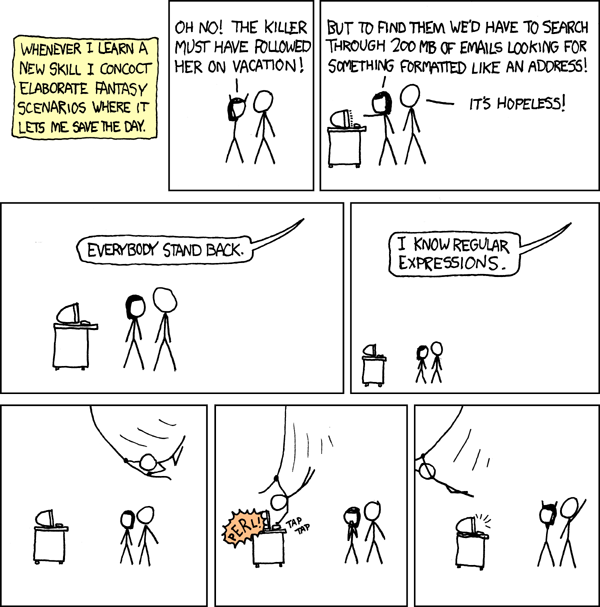
\includegraphics[scale=.3]{img/regular_expressions.png}
    \end{figure}
\end{frame}

\appendix
\beginbackup

\begin{frame}{Fragen?}
    \begin{figure}
        
\includegraphics[scale=.6]{img/formulas.png}
    \end{figure}
\end{frame}

\begin{frame}{Bonus Track: Stack Sort}
    \url{https://gkoberger.github.io/stacksort}
\end{frame}

\begin{frame}{Bis nächste Woche!}
    \begin{figure}
        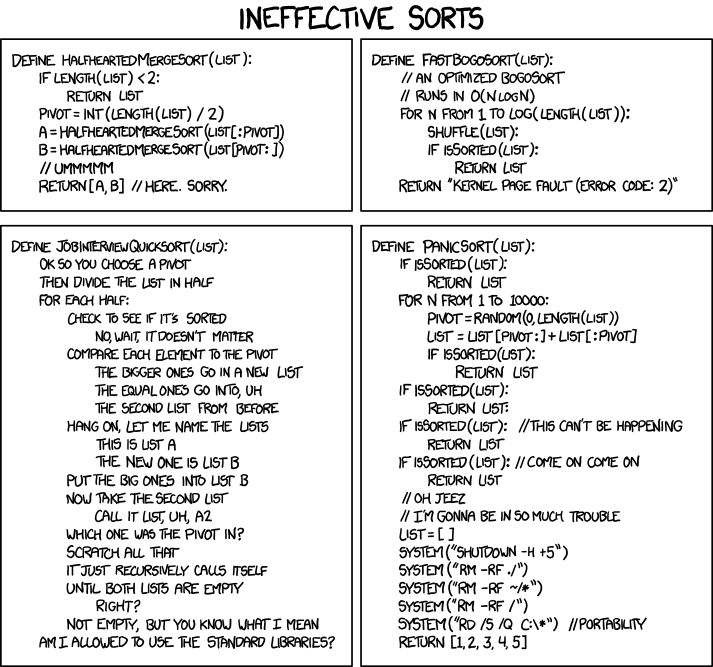
\includegraphics[scale=.3]{img/ineffective_sorts.png}
        \caption{\footnotesize{xkcd.com}}
    \end{figure}
\end{frame}

\backupend

\end{document}
